\chapter{Raspberry Piをリモコンにしてみよう}
\section{はじめに}
\subsection{この章で学ぶこと}

この章では以下のことを学びます。
\begin{itemize}
\item FaBoの\ruby{操作}{そう|さ}
\item 赤外線の信号の送り方
\end{itemize}

「FaBoの操作」では、いろいろなセンサーをRaspberry Piに\ruby{接続}{せつ|ぞく}して、どのようなデータを入力できるのか、どのようなデータを出力できるのかを学びます。また、センサーのデータをプログラムで利用したり、プログラムで指定したデータを出力装置から出力する方法を学びます。

「赤外線の信号の送り方」では、赤外線とは何か、赤外線リモコンの信号の読み取りかた、赤外線リモコンの信号の出力の仕方を学びます。また、プログラムからリモコンの信号を送信する方法を学びます。

\subsection{教材を自分のフォルダに置こう}
まずは、今回利用する教材をコピーしましょう。
これまでの回と同じように、\nobreak/usr/local/share/ome あるディレクトリ 05 をホームディレクトリにコピーしましょう。

\newpage
\section{センサーの\ruby{基本}{き|ほん}}
\subsection{センサーってなんだろう?}
センサーは身の回りの世界の\ruby{情報}{じょう|ほう}を調べ、コンピュータに伝えるための装置です。明るさ、温度、\ruby{湿度}{しつ|ど}を調べることができるセンサーボードは第3回の\ruby{授業}{じゅ|ぎょう}で\ruby{扱}{あつか}いました。しかし、センサーはたくさんの種類があり、出来ることももっとたくさんあります。まず、車で使われているセンサーを見てみましょう。
\begin{figure}[htb]
\begin{center}
    \includesvg[width=0.7\linewidth]{images/chap05/car_sensors.svg}
    \caption{自動車に使われているセンサー}
    \label{fig1}
\end{center}
\end{figure}
\begin{table}[htb]
  \caption{自動車に使われているセンサーの種類とできること}
  \label{table-sensors}
  \centering
  \begin{widerrows}[1.3] 
    \begin{tabular}{|l|l|} \hline
      \multicolumn{1}{|c|}{センサーの種類} & \multicolumn{1}{c|}{できること} \\ \hline\hline
      赤外線カメラ & \ruby{暗闇}{くら|やみ}で物を見ることができる \\
      ステアリングセンサ & ハンドルの回し具合によってタイヤの方向を決める \\
      \ruby{圧力}{あつ|りょく}センサ & 圧力を調べる \\
      アクセルセンサ & アクセルペダルの\ruby{踏}{ふ}み具合を調べる \\
      ミリ波レーダー & 車の前に物があるかを調べる \\
      トルクセンサ & ねじれの強さを調べる \\
      $O_2$センサ & \ruby{燃料}{ねん|りょう}の働き具合を空気の\ruby{酸素}{さん|そ}($O_2$)量で調べる \\
      ホイール速度センサ & タイヤの回転速度を調べる \\
      ヨーレートセンサ&加速度センサ & 車の速さを調べる \\
      車間\ruby{制御}{せい|ぎょ}センサ & 前の車との\ruby{距離}{きょ|り}を調べる \\
      エアバックセンサ & 車の\ruby{衝突}{しょう|とつ}を感知して\ruby{瞬時}{しゅん|じ}にエアバッグを\ruby{膨}{ふく}らませる \\ \hline
    \end{tabular}
  \end{widerrows} 
\end{table}

このように、機械では多くのセンサーが使われています。今日の授業ではセンサーをいくつか扱います。どのセンサーが何に使えそうか、何に使われていそうかを考えながら使ってみましょう。

\subsection{アナログ信号とデジタル信号}
センサーが出力するデータは大きく分けて2種類あり、デジタル信号とアナログ信号と\ruby{呼}{よ}ばれる信号のどちらを使うかで分けられています。2つの信号には以下の図のような\ruby{違}{ちが}いがあります。
\begin{figure}[htbp]
  \begin{minipage}[b]{0.5\linewidth}
    \centering
    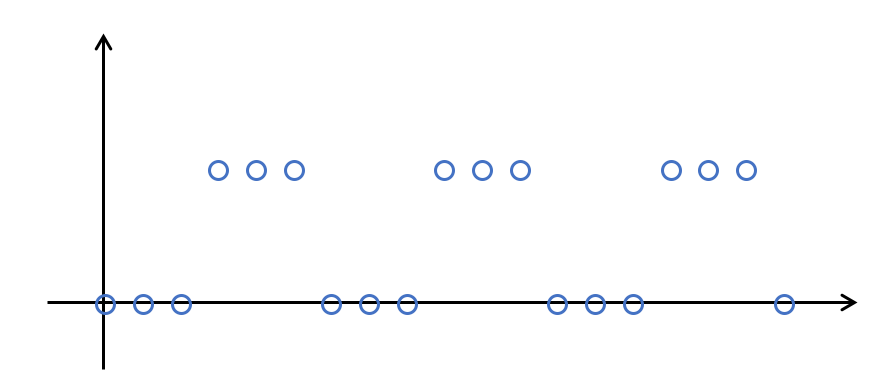
\includegraphics[keepaspectratio, scale=0.5]{images/chap05/text05-img002.png}
    \caption{デジタル信号の例}
    \label{fig2}
  \end{minipage}
  \begin{minipage}[b]{0.5\linewidth}
    \centering
    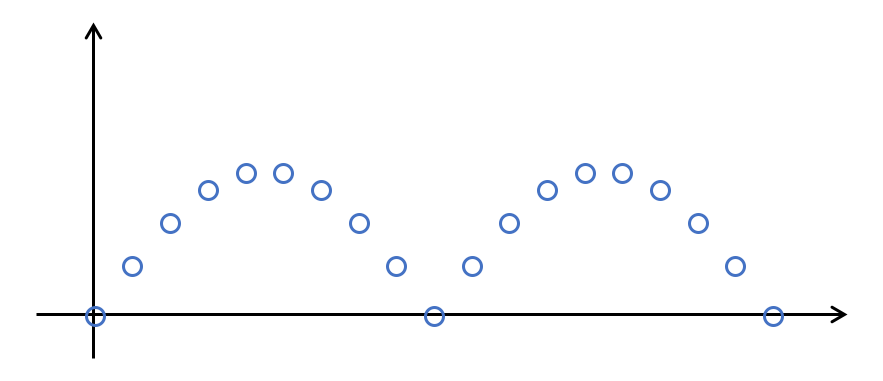
\includegraphics[keepaspectratio, scale=0.5]{images/chap05/text05-img003.png}
    \caption{アナログ信号の例}
    \label{fig3}
  \end{minipage}
\end{figure}

図\ref{fig2}と図\ref{fig3}はコンピュータで使われている信号をグラフにしたものです。授業で使用するセンサーのデジタル信号は、図\ref{fig2}と図\ref{fig3}のように2種類の\ruby{値}{あたい}を表すことができます。2種類の値は0か1です。一方授業で使用するアナログ信号は、\ref{fig3}のように中間の値を表すことができます。この値は0〜1023の数字で\ruby{表現}{ひょう|げん}されます。

デジタル信号はボタンが\ruby{押}{お}されたか押されていないか、明かりがついたか消えたかなどのふた通りのものを表すときに使われ、アナログ信号は主に明るさや距離などの数を表すときに使われます。

\begin{tcolorbox}[title=\useOmetoi]
  \begin{enumerate}
  \addquiz{センサーとはなんだろう。説明してみましょう。}
  \addquiz{車で使われているセンサーを3つ書いてみましょう。}
  \addquiz{アナログ信号、デジタル信号の違いを書いてみましょう。}
\end{enumerate}
\end{tcolorbox}
